\documentclass[pdflatex,compress]{beamer}

%\usetheme[dark,framenumber,totalframenumber]{ElektroITK}
\usetheme[darktitle,framenumber,totalframenumber]{ElektroITK}

\usepackage{graphicx}

\title{PEMODELAN JARINGAN KOMUNIKASI}
\subtitle{IP Address Classes}

\author{Mifta Nur Farid, S.T., M.T.}

\begin{document}

\maketitle

\section{Class A IP Addresses}

\begin{frame}{Subnet Size}
	\begin{center}
		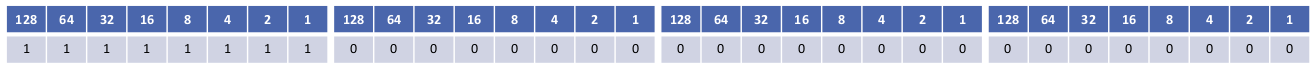
\includegraphics[width=1\linewidth]{img/img01}
	\end{center}
	\begin{itemize}
		\item The bigger the host portion of the network, the more hosts we can have
		\item If the subnet mask is /8, we have 24 bits available to allocate to hosts
		\item If the subnet mask is /24, we only have 8 bits available to allocate to hosts
	\end{itemize}
\end{frame}

\begin{frame}{How Internet Addressing Was Meant to Work}
	\begin{itemize}
		\item The global coordination of Internet IPv4 addressing is performed by IANA (Internet Assigned Numbers Authority).
		\item This is the way it was originally supposed to work:
		\item When a company wants to communicate on the internet, they apply for a range of IP addresses.
		\item If they have 6000 hosts, they ask for a range of IP addresses big enough to cover that, plus room for growth.
		\item They then allocate their addresses to their hosts in their various offices.
	\end{itemize}
\end{frame}

\begin{frame}{How Internet Addressing Was Meant to Work}
	\begin{itemize}
		\item Unfortunately, when IPv4 was created, the designers didn't realise how big the internet was going to get, and they didn't create a big enough address space - there's not enough addresses for everyone.
		\item The long term solution to this problem is IPv6 which has a much bigger address space.
	\end{itemize}
\end{frame}

\end{document}